\chapter{Kết quả huấn luyện và đánh giá}
\section{Kết quả huấn luyện}
Với các thông số mạng đã cấu hình ở chương trước, \ref{fig:res} cho thấy kết quả huấn sau khi huấn luyện mạng có kết quả tương đối tốt với giá trị \(cross_entropy = 0.29\) và độ chính xác ở tập kiểm thử là 88.7\%. Không những thế việc áp dụng kỹ thuật transfer learning giúp tiết kiệm thời gian huấn luyện gấp nhiều lần. Cụ thể, việc xây dựng mô hình thủ công và huấn luyện lại từ đầu đối với máy tính không hỗ trợ card GPU sẽ mất thời gian là 8 tiếng nhưng đối với việc áp dụng mô hình inception model với kỹ thuật transfer learning thì chỉ mất từ 45 đến 60 phút để hoàn thành.\par
\pagebreak
	\begin{figure}[h!]
		\centering
		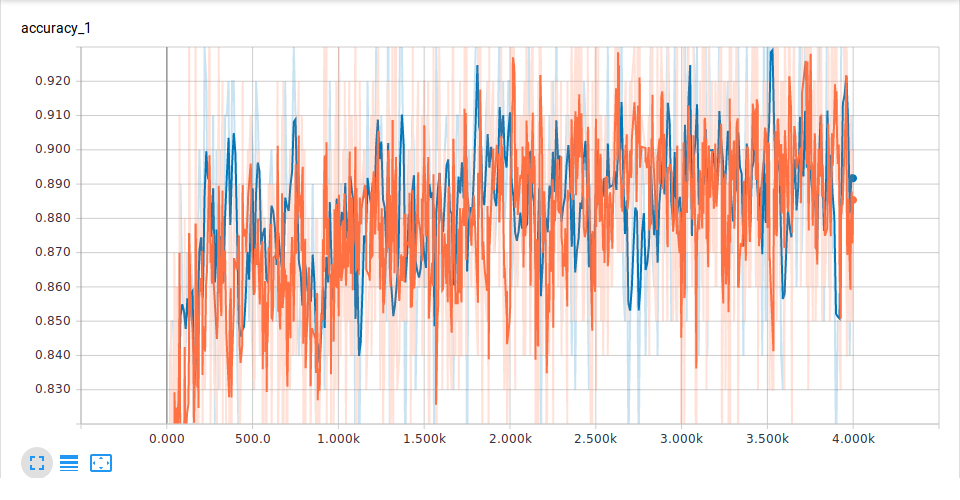
\includegraphics[scale=0.5]{charts/accuracy.png}
		\caption{Đồ thị biểu diễn độ chính xác (accuracy)}
		\label{fig:accuracy}
	\end{figure}

Đồ thị \ref{fig:accuracy} biểu diễn chi tiết độ chính xác trong quá trình huấn luyện với đường màu cam biểu diễn cho quá trình huấn luyện và đường màu xanh lam biểu diễn cho kiểm tra trên tập Validation. Tương tự với \ref{fig:cross_entropy}.
	\pagebreak
	\begin{figure}[h!]
		\centering
		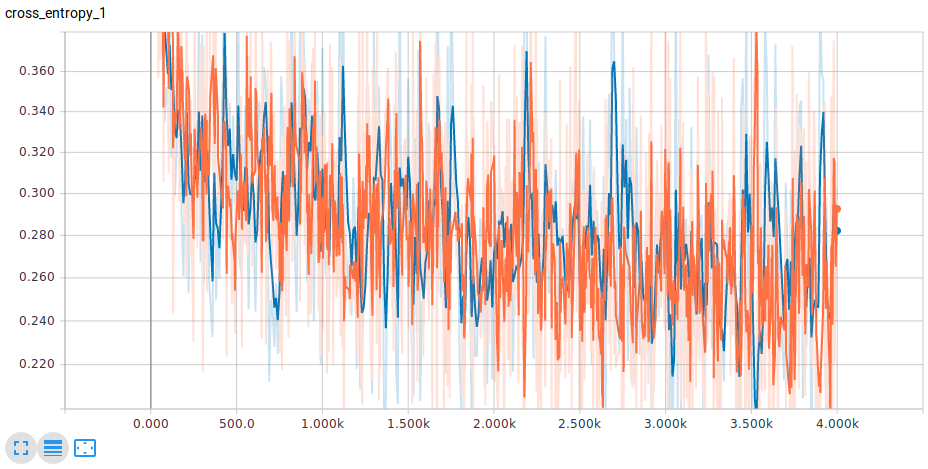
\includegraphics[scale=0.5]{charts/cross-entropy.png}
		\caption{Đồ thị biểu diễn độ sai số (cross entropy)}
		\label{fig:cross_entropy}
	\end{figure}

\section{Sử dụng mô hình phân loại ảnh mới}
	Sử dụng mô hình để phân loại một số hình ảnh khác chưa được phân loại. \ref{fig:test1} và \ref{fig:test2} có thể nhận biết bằng mắt thường đây là hình ảnh của những con đường đang trong tình trạng ùn tắt. Kết quả dự đoán cho lớp cả hai hình ảnh này là chính xác theo lớp kẹt xe.
	\pagebreak
	
	\begin{figure}[h!]
		\centering
		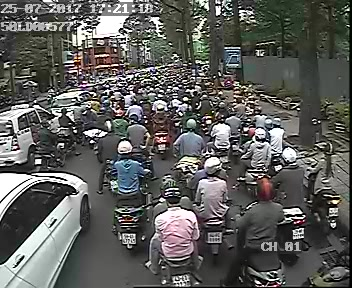
\includegraphics[scale=1]{charts/test-ket.jpg}
		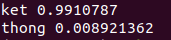
\includegraphics[scale=0.5]{charts/test-ket-res.png}
		\caption{Ảnh kiểm thử 1 - kết quả}
		\label{fig:test1}
	\end{figure}
	
	\begin{figure}[h!]
		\centering
		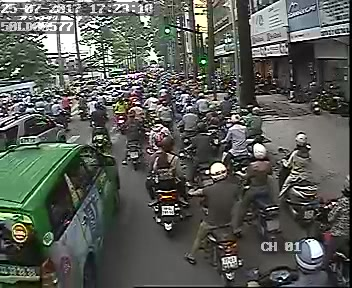
\includegraphics[scale=1]{charts/test-ket1.jpg}
		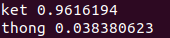
\includegraphics[scale=0.5]{charts/test-ket1-res.png}
		\caption{Ảnh kiểm thử 2 - kết quả}
		\label{fig:test2}
	\end{figure}
	
	\pagebreak
	Đối với hai hình ảnh tiếp theo được phân biệt vào loại đường thông thoáng một cách dễ dàng. Mô hình dự đoán xác suất hai hình ảnh dưới đây thuộc lớp thông thoáng lần lượt là.
	\pagebreak
	\begin{figure}[h!]
		\centering
		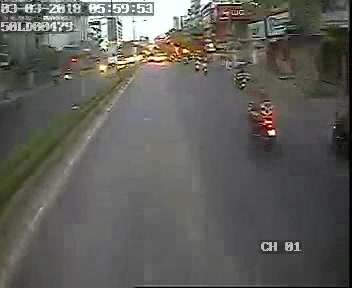
\includegraphics[scale=1]{charts/image0125.jpg}
		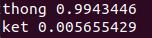
\includegraphics[scale=0.5]{charts/most-last-res.png}
		\caption{Ảnh kiểm thử 3 - kết quả}
		\label{fig:test3}
	\end{figure}
	
	
	\begin{figure}[h!]
		\centering
		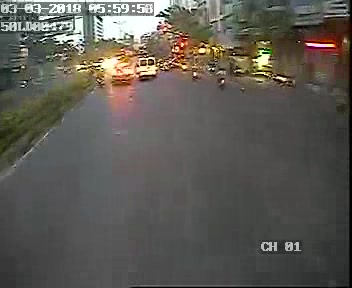
\includegraphics[scale=1]{charts/image0126.jpg}
		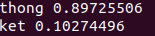
\includegraphics[scale=0.5]{charts/last-res.png}
		\caption{Ảnh kiểm thử 4 - kết quả}
		\label{fig:test4}
	\end{figure}
	\pagebreak
	Như vậy, kết quả kiểm thử đối với một số hình ảnh chưa được phân loại của mô hình đã huấn luyện cho kết quả khá chính xác. Tuy nhiên, đối với vấn đề  phân loại giao thông thì không chỉ có hai trường hợp ùn tắt hay thông thoáng mà còn tồn tại nhiều trường hợp hơn. Như tình huống đông xe nhưng di chuyển chậm, trên thực tế đây là tình huống không phải ùn tắt nhưng ảnh chụp gần giống với ảnh ùn tắt. Cần chú ý vấn đề này khi lựa chọn, phân loại ảnh huấn luyện, hoặc để giải quyết tốt hơn cần phải tăng số lượng lớp(nhãn) cần phân loại lên thành 3 hay lớn hơn thay vì 2 như ban đầu.
	
	
	